\documentclass[tikz,border=10pt]{standalone}

% Use the Atkinson Hyperlegible font with sfdefault option to make it the main text font
\usepackage[sfdefault]{atkinson}

\usepackage{tikz}
\usetikzlibrary{arrows.meta, positioning, shapes, calc, fit}

\begin{document}


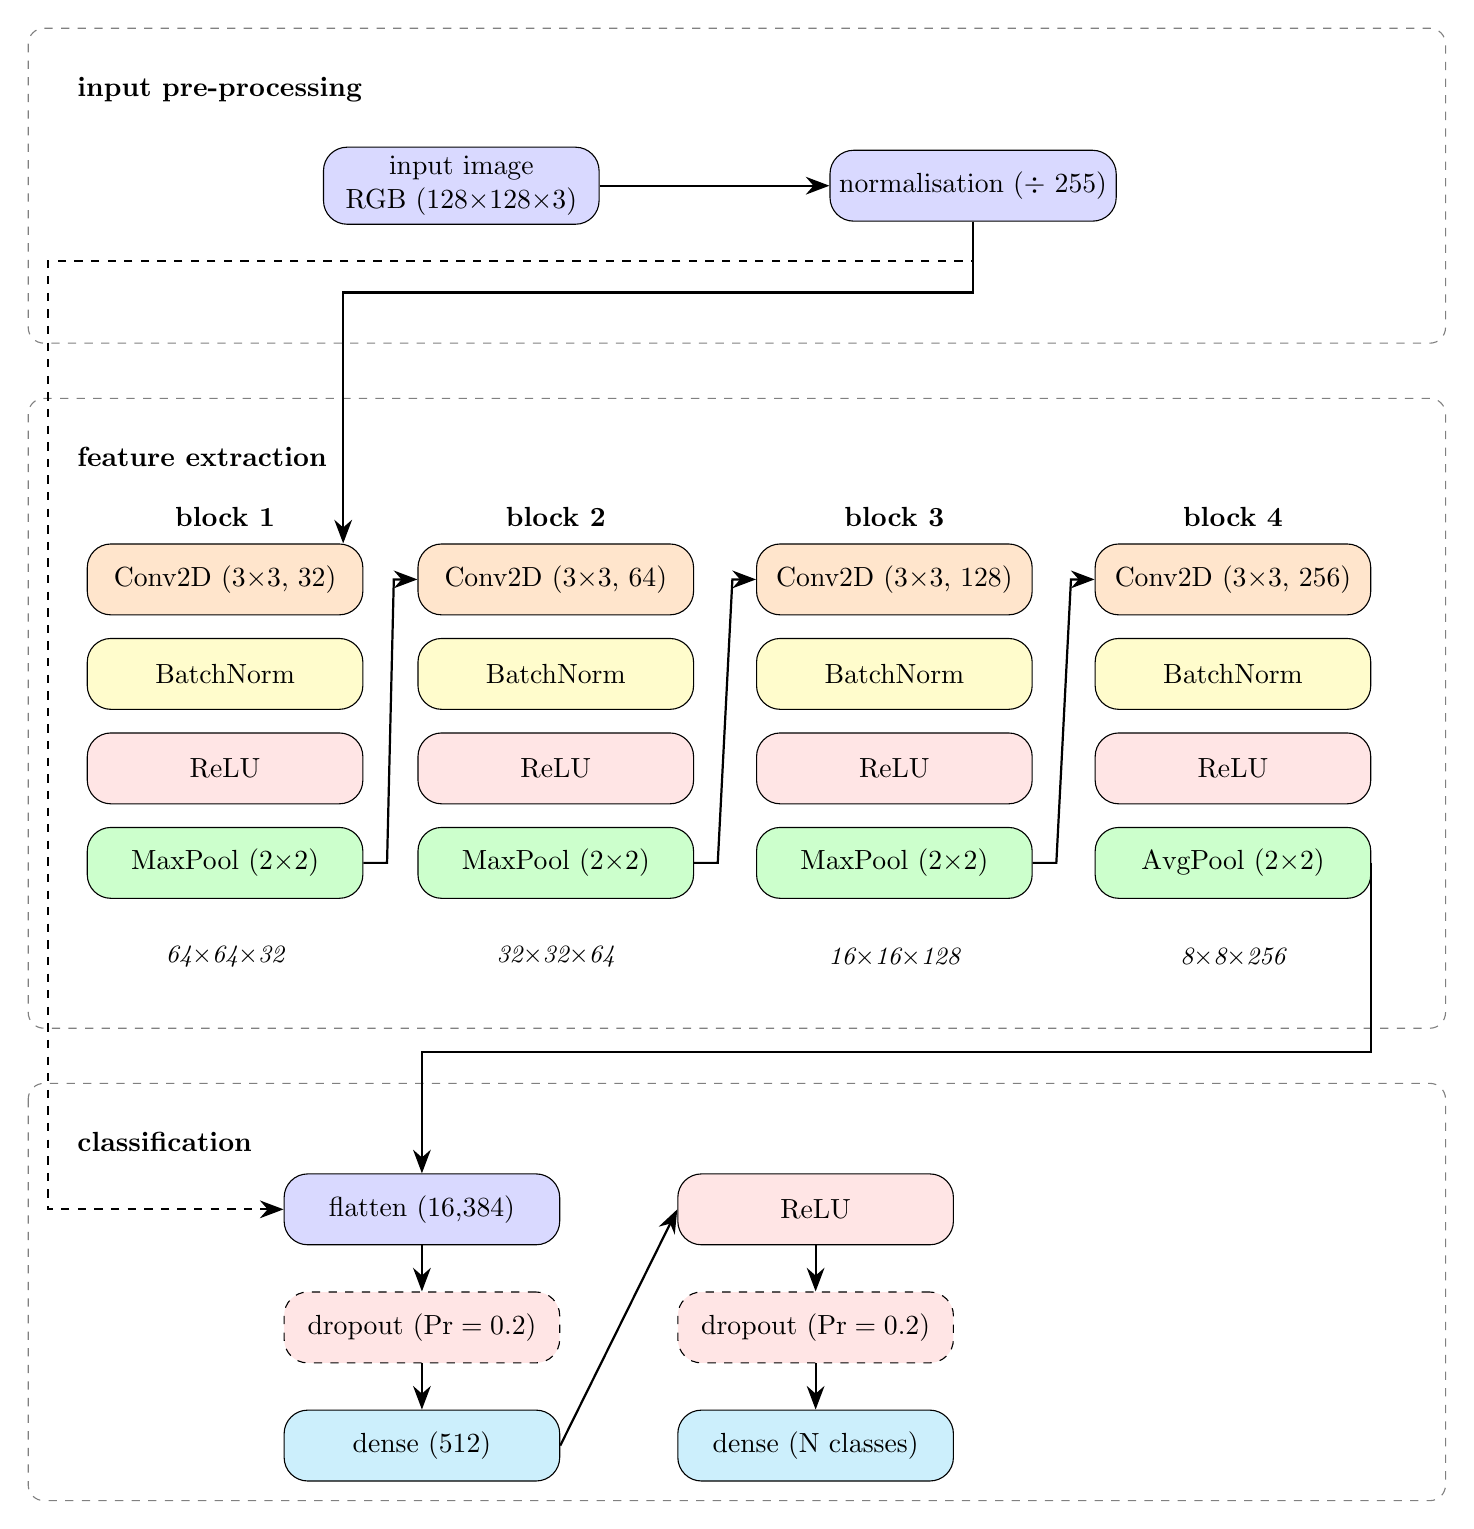
\begin{tikzpicture}[
  % Define styles for different elements
  box/.style={draw, rounded corners=3mm, minimum width=3.5cm, minimum height=0.9cm, align=center},
  inputbox/.style={box, fill=blue!15},
  convbox/.style={box, fill=orange!20},
  batchbox/.style={box, fill=yellow!20},
  relubox/.style={box, fill=red!10},
  poolbox/.style={box, fill=green!20},
  dropbox/.style={box, fill=red!10, dashed},
  densebox/.style={box, fill=cyan!20},
  arrow/.style={-{Stealth[length=3mm]}, thick},
  skiparrow/.style={-{Stealth[length=3mm]}, thick, dashed},
  block/.style={draw=gray, dashed, rounded corners=2mm, inner sep=0.3cm},
  title/.style={font=\Large\bfseries},
  subtitle/.style={font=\bfseries, align=left},
  dims/.style={font=\small\itshape}
]

% Row 1: Input Preprocessing
\coordinate (feat_top_left) at (-9, 0);
\coordinate (feat_top_right) at (9, 0);
\coordinate (feat_bot_left) at (-9, -4);
\coordinate (feat_bot_right) at (9, -4);

\draw[gray, dashed, rounded corners=2mm] (feat_top_left) rectangle (feat_bot_right);
\node[subtitle, anchor=north west] at ($(feat_top_left) + (0.5,-0.5)$) {input pre-processing};

\node[inputbox] (input) at (-3.5,-2) {input image\\RGB (128$\times$128$\times$3)};
\node[inputbox] (norm) at (3,-2) {normalisation ($\div$ 255)};

\draw[arrow] (input) -- (norm);

% Row 2: Feature Extraction
\coordinate (blocks_top_left) at (-9, -4.7);
\coordinate (blocks_top_right) at (9, -4.7);
\coordinate (blocks_bot_left) at (-9, -12.7);
\coordinate (blocks_bot_right) at (9, -12.7);

\draw[gray, dashed, rounded corners=2mm] (blocks_top_left) rectangle (blocks_bot_right);

% Fixed Feature Extraction label - properly positioned and separate from Block 1
\node[subtitle, anchor=north west] at ($(blocks_top_left) + (0.5,-0.5)$) {feature extraction};

% Block labels - moved Block 1 label down to avoid overlap
\node[subtitle] at (-6.5, -6.2) {block 1};
\node[subtitle] at (-2.3, -6.2) {block 2};
\node[subtitle] at (2, -6.2) {block 3};
\node[subtitle] at (6.3, -6.2) {block 4};

% Block 1 Components
\node[convbox] (conv1) at (-6.5, -7) {Conv2D (3$\times$3, 32)};
\node[batchbox] (bn1) at (-6.5, -8.2) {BatchNorm};
\node[relubox] (relu1) at (-6.5, -9.4) {ReLU};
\node[poolbox] (pool1) at (-6.5, -10.6) {MaxPool (2$\times$2)};
\node[dims] (dims1) at (-6.5, -11.8) {64$\times$64$\times$32};

% Block 2 Components
\node[convbox] (conv2) at (-2.3, -7) {Conv2D (3$\times$3, 64)};
\node[batchbox] (bn2) at (-2.3, -8.2) {BatchNorm};
\node[relubox] (relu2) at (-2.3, -9.4) {ReLU};
\node[poolbox] (pool2) at (-2.3, -10.6) {MaxPool (2$\times$2)};
\node[dims] (dims2) at (-2.3, -11.8) {32$\times$32$\times$64};

% Block 3 Components
\node[convbox] (conv3) at (2, -7) {Conv2D (3$\times$3, 128)};
\node[batchbox] (bn3) at (2, -8.2) {BatchNorm};
\node[relubox] (relu3) at (2, -9.4) {ReLU};
\node[poolbox] (pool3) at (2, -10.6) {MaxPool (2$\times$2)};
\node[dims] (dims3) at (2, -11.8) {16$\times$16$\times$128};

% Block 4 Components
\node[convbox] (conv4) at (6.3, -7) {Conv2D (3$\times$3, 256)};
\node[batchbox] (bn4) at (6.3, -8.2) {BatchNorm};
\node[relubox] (relu4) at (6.3, -9.4) {ReLU};
\node[poolbox] (pool4) at (6.3, -10.6) {AvgPool (2$\times$2)};
\node[dims] (dims4) at (6.3, -11.8) {8$\times$8$\times$256};

% Row 3: Classification
\coordinate (class_top_left) at (-9, -13.4);
\coordinate (class_top_right) at (9, -13.4);
\coordinate (class_bot_left) at (-9, -18.7);
\coordinate (class_bot_right) at (9, -18.7);

\draw[gray, dashed, rounded corners=2mm] (class_top_left) rectangle (class_bot_right);
\node[subtitle, anchor=north west] at ($(class_top_left) + (0.5,-0.5)$) {classification};

% Two-column layout for classification components
\node[inputbox] (flatten) at (-4, -15) {flatten (16,384)};
\node[dropbox] (dropout1) at (-4, -16.5) {dropout ($\Pr = 0.2$)};
\node[densebox] (dense1) at (-4, -18) {dense (512)};

\node[relubox] (relu5) at (1, -15) {ReLU};
\node[dropbox] (dropout2) at (1, -16.5) {dropout ($\Pr = 0.2$)};
\node[densebox] (dense2) at (1, -18) {dense (N classes)};

% From Normalisation to Block 1
\draw[arrow] (norm.south) -- ++(0,-0.9) -- ++(-8, 0) -- ($(conv1.north) + (1.5, 0)$);

% Diagonal arrows that don't intersect nodes
\coordinate (pool1_right) at ($(pool1.east) + (0.3,0)$);
\coordinate (conv2_left) at ($(conv2.west) - (0.3,0)$);
\coordinate (pool2_right) at ($(pool2.east) + (0.3,0)$);
\coordinate (conv3_left) at ($(conv3.west) - (0.3,0)$);
\coordinate (pool3_right) at ($(pool3.east) + (0.3,0)$);
\coordinate (conv4_left) at ($(conv4.west) - (0.3,0)$);

\draw[arrow] (pool1) -- (pool1_right) -- ($(pool1_right)!0.5!(conv2_left) + (0,0)$) -- (conv2_left) -- (conv2);
\draw[arrow] (pool2) -- (pool2_right) -- ($(pool2_right)!0.5!(conv3_left) + (0,0)$) -- (conv3_left) -- (conv3);
\draw[arrow] (pool3) -- (pool3_right) -- ($(pool3_right)!0.5!(conv4_left) + (0,0)$) -- (conv4_left) -- (conv4);

% Connection from AvgPool to Flatten
\draw[arrow] (pool4.east) -- ++(0,-2.4) -| (flatten.north);

% Skip connection from Normalisation to Classification
\draw[skiparrow] (norm.south) -- ++(0,-0.5) -| ($(blocks_top_left) + (0.25,0)$) -- ($(-9, -15) + (0.25,0)$) -- (flatten.west);

% Arrows for classification section
\draw[arrow] (flatten.south) -- (dropout1.north);
\draw[arrow] (dropout1.south) -- (dense1.north);
\draw[arrow] (dense1.east) -- (relu5.west);
\draw[arrow] (relu5.south) -- (dropout2.north);
\draw[arrow] (dropout2.south) -- (dense2.north);

\end{tikzpicture}

\end{document}